% !TeX program = lualatex
\documentclass[3pt,landscape]{article}
\usepackage{multicol, calc, ifthen, amsmath, amsthm, amsfonts, amssymb, color, graphicx, overpic, hyperref, fontspec, xunicode}

\usepackage[landscape]{geometry}

\defaultfontfeatures{Mapping=tex-text,Scale=MatchLowercase}
\ifthenelse{\lengthtest { \paperwidth = 11in}}
    { \geometry{top=.3in,left=.3in,right=.3in,bottom=.3in} }
    {\ifthenelse{ \lengthtest{ \paperwidth = 297mm}}
        {\geometry{top=1cm,left=1cm,right=1cm,bottom=1cm} }
        {\geometry{top=1cm,left=1cm,right=1cm,bottom=1cm} }
    }
\pagestyle{empty}
\makeatletter
\setmainfont{Source Sans Pro}
\setmonofont{Menlo}
\DeclareMathSizes{3}{3}{2}{1}

\renewcommand{\section}{\@startsection{section}{1}{0mm}{-1ex plus -.5ex minus -.2ex}{0.5ex plus .2ex}{\normalfont\large\bfseries}}
\renewcommand{\subsection}{\@startsection{subsection}{2}{0mm}{-1explus -.5ex minus -.2ex}{0.5ex plus .2ex}{\normalfont\normalsize\bfseries}}
\renewcommand{\subsubsection}{\@startsection{subsubsection}{3}{0mm}{-1ex plus -.5ex minus -.2ex}{1ex plus .2ex}{\normalfont\small\bfseries}}
\makeatother
\setcounter{secnumdepth}{0}
\setlength{\parindent}{0pt}
\setlength{\parskip}{0pt plus 0.5ex}
\hypersetup{colorlinks=true, urlcolor=blue}
\def\ci{\perp\!\!\!\perp}

%%%%%%%%%%%%%%%%%%%%%%%%%%%%%%%%%%%%%%%%%%%%%%%%%%

\begin{document}
\raggedright
\footnotesize

\begin{multicols}{3}
\setlength{\premulticols}{1pt}
\setlength{\postmulticols}{1pt}
\setlength{\multicolsep}{1pt}
\setlength{\columnsep}{2pt}

\begin{center}
    \Large{\underline{Algorithms Mini Field Guide 1.4}} \\
\end{center}
\begin{center}
    Written by: \href{http://krishna.im}{Krishna Parashar}\\
    Published by: \href{http://www.ocm.io}{The OCM}\\
\end{center}

%%%%%%%%%%%%%%%%%%%%%%%%%

\section*{Huffman Encoding}
A means to encode data using the optimal number of bits for each character given a distribution.
\begin{verbatim}
func huffman(f):
    Input: An array f[1...n] of frequencies
    Output: An encoding tree with n leaves

    let H be a priority queue of integers, ordered by f
    for i=1 to n: insert(H,i)
    for k = n+1 to 2n-1:
        i=deletemin(H), j=deletemin(H)
        create a node numbered k with children i,j
        f[k] = f[i]+f[j]
        insert(H,k)
\end{verbatim}

%%%%%%%%%%%%%%%%%%%%%%%%%

%\section*{Amortized Analysis}

%%%%%%%%%%%%%%%%%%%%%%%%%

\section*{Dynamic Programming}
Fundamentally DP is carefully bruteforcing the solutions to a problem by turning it into smaller and smaller nested subproblems that remember useful information about its bigger or parent subproblem so that it can eventually reconstruct itself to solve the original problem in a reasonable amount of time. This ``remembrance'' is often done using memoization or parent pointers.\\
Dynamic Programming has two approaches, which both have the same asymptotic runtime (differ by a constant):
\begin{enumerate}
\item \textbf{Top Down:}
The top down approach uses the recursive idea of breaking the problem into trivially (but still helpful) smaller subproblems and finding a way (through brute force and memorization) to find the maximum or minimum of every permutation what is be left with ever permutation of the subproblems. This is unlike Divide and Conquer which garners its efficiency from reducing its subproblems to massively smaller problems. 
\item \textbf{Bottom Up:}
The bottom up approach uses the opposite approach of breaking down the problem into its smallest subproblems and iteratively using the smaller problems to solve bigger and bigger problems until it solves the original problem. A table is often used to keep track of these values. BU is more space efficient than TD, unless you use tail recursion for TD.
\end{enumerate} 
You can solve most DP problems by the following steps:
\begin{enumerate}
\item Define the subproblems. Know the \# of subproblems. 
\item Guess a solution for what is not the subproblem (max/min of brute force permutations). Know the \# of guesses.
\item Relate the subproblems to the parent problem. This is the recursive/iterative step. 
\item Do the recursion and memoize or iteratively build a table to keep track of previously used values. These can be used to form a DAG. Ensure the DAG for these are acyclic (i.e. have valid topological order or no dependences on parent problems)
\item Solve the original problem
($\theta(\# subproblems * time/subproblem)$)
\end{enumerate} 
Choosing Subproblems ($i$ is current problem):
\begin{itemize}
\item \textbf{Suffix: } $x[i:] \forall i$ - $O(n)$ (subproblems are broken from i to end)
Topological Order is right to left. 
\item \textbf{Prefix: } $x[:i] \forall i$ - $O(n)$ (subproblems are broken from start to i)
Topological Order is left to right. 
\item \textbf{Substrings: } $x[i:j] \forall i,j$ - $O(n^2)$ (subproblems are fragments of problem, combination of suffix and prefix)
Topological Order is increasing substring size. 
\end{itemize}



\subsection*{Fibonacci \(O(n)\)}
\textbf{Recursive:}
\begin{verbatim}
memo = {}
fib(n):
    if n in memo: return memo[n]
    if n <= 2: f = 2
    else: f = fib(n-1) + fib(n-2)
    memo[n] = f
    return f
\end{verbatim}
\textbf{Iterative:}
\begin{verbatim}
fib = []
fib(n):
    for k in range(1, n):
        if k <= 2: f = 2
        else: f = fib[k-1] + fib[n-2]
        fib[k] = f
    return fib[n]
\end{verbatim}
\subsection*{Shortest Paths $\theta(VE)$}
\textbf{For DAGs:}
For a shortest path (s,v) that uses a limit of, guess take the min of the incoming edge weights into v, say from a node u and then add it to the prefix subproblem of shortest path from (s, u).\\
\textbf{For General: }
$S_k (s, v) = $ weight of shortest path from s to v that uses $\le k$ edges.
$S_k (s, v) = min_{(u, v) in E}(S_{k-1} (s, u) + w(u, v)$\\
This is Bellman-Ford. 

\subsection*{Longest Increasing Subsequence: \(O(n^{2})\)}
Please note that subsequences are any sequences found in another sequences that are not necessarily next to each other (contiguous). Contiguous subsequences are substrings. 
The following algorithm starts at one side of the list and finds the max length of sequences terminating at that given node, recursively following backlinks. Then given all the lengths of paths terminating at that given node choose the max length. Without memoization, this solution would be exponential time.
\begin{verbatim}
L = {}
for j=1,2,...,n:
    L[j] = 1+max{L[i]:(i,j) in E}
    # The (i,j) represents all the edges that go from
    # a node to j.
return max(L)
\end{verbatim}

\subsection*{Edit Distance (Spelling Suggestions)}
This algorithm works by basically choosing the min of the options for every given letter. (The 3 options being adding a gap inbetween letters of one of the strings or matching the two letters and moving on.)\\
ex) Snowy and Sunny have an edit distance of 3 with this configuration
\begin{verbatim}
S _ N O W Y
S U N N _ Y
\end{verbatim}
\begin{verbatim}
for i = 0,1,2,...,m:
    E(i,0) = i
for j = 1,2,...,n:
    E(0,j) = j
for i = 1,2,...,m:
    for j = 1,2,...,n:
        E(i,j) = min{E(i-1,j)+1,E(i,j-1)+1,E(i-1,j-1)
                    +diff(i,j)}
return E(m,n)
\end{verbatim}

\subsection*{Knapsack \(O(nW)\)}
Items have a weight and a value, you want to maximize the value within a given weight. (The amount you can carry in your knapsack)\\
With repetition:
\[K(\omega)=max_{\texttt{items}}\{K(\omega-\omega_{\texttt{item}})+value\}\]
Without repetition:
\[K(\omega,j)=max_{\texttt{available items}}\{K(\omega-\omega_{j},j-1)+V_{j},k(\omega, j-1)\}\]

\subsection*{Parenthesization \(O(n^3)\)}
\[C(i,j)=min\{C(i,k)+c(k+1,j)+m_{i-1}\cdot m_{k} \cdot m_{j}\}\]

\subsection*{Floyd-Warshall \(O(|V|^{3})\)}
Used for finding shortest paths in a weighted graph with positive or negative edge weights (but with no negative cycles/
\begin{verbatim}
for i=1 to n:
    for j=1 to n:
        dist(i,j,0) = infinity
    for all (i,j) in E:
        dist(i,j,0) = l(i,j)
for k = 1 to n:
    for i = 1 to n:
        for j = 1 to n:
            dist(i,j,k) = min{dist(i,k,k-1)+
                              dist(k,j,k-1),
                              dist(i,j,k-1)}
\end{verbatim}

\subsection*{Traveling Salesman Problem (TSP) \(O(n^{2}2^{n})\)}
Shortest path for visiting all nodes. 
\begin{verbatim}
C({1},1)=0
for s = 2 to n:
    for all subsets S in {1,2,...,n} of size s and has l:
        C(S,1) = infinity
        for all j in S,j != 1:
            C(S,j) = min{C(S-{j},i)+dij:i in S,i not in j}
return min over j, C({1,...,n},j)+dj1
\end{verbatim}

%%%%%%%%%%%%%%%%%%%%%%%%%

\section*{Linear Programming}
Feed into a LP solver like Simplex an \textit{Objective Function} which states if you want to maximize or minimize the equation (max$(x+2y)$), \textit{Constraints} which are limitations for the variables of the Objective Function ($x \ge 0, y \le 600$).
\begin{enumerate}
    \item To turn a maximization problem into a minimization (or vice versa) just multiply the coeficients of the objective function by -1.
    \item To turn an inequality constraint like \(\sum_{i=1}^{n}a_i x_i \leq b\) into an equation, introduce a new variable S and use, \(\sum^n_{i=1}a_{i}x_{i}+s = b\), \(s \geq 0\) (S is known as a slack variable)
    \item To change an inequality constraint into inequalities rewrite \(ax=b\),\\
        as \(ax \leq b \texttt{ and } ax \geq b\)
    \item If a linear program has an unbounded value then its dual must be infeasible.
\end{enumerate}


\subsection*{Max Flow}
Construct graph G that is a simple directed graph with source s and sink t. No negative capacities are possible.\\
Construct a Residual Graph with forward edges for the amount of capacity that is not being used (capacity - current use) and a back edge for what is currently being used. 

\subsubsection*{Ford-Fulkerson}
Start with no flow on your graph. Find a path using DFS. Then create a residual graph. We can now use DFS for finding a path from s to t in the residual graph. If one exists we are not optimally using our flow. We then find the edge with the LEAST capacity edge - this is our bottleneck - and add flow onto all the edges in that path up to the capacity that is not being used by the bottleneck edge, hereby maximizing the flow of the path. Our new flow is guaranteed to be better. Create a new residual graph and repeat until no path in the residual graph can be found from s to t. This will happen when capacity = current use, as we lose our forward edge and only have a back edge.\\
This algorithm will sometimes decrease flow in one area to increase flow in another. Max flow is the total weights of incoming edges to the sink. Runtime would be $O(E * M)$, where $M$ is the number of iterations and $E$ is the time to find a path. This can also be stated as $O($maxflow$*E)$. However this may not terminate. If you use BFS instead of DFS you are using the Edmonds-Karp Algorithm which will terminate and has complexity $O(V*(E)^2)$, which is better for large networks.
\begin{center}
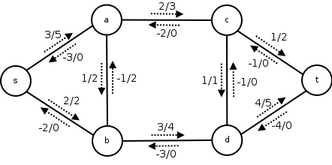
\includegraphics[scale=.25]{flow.png}
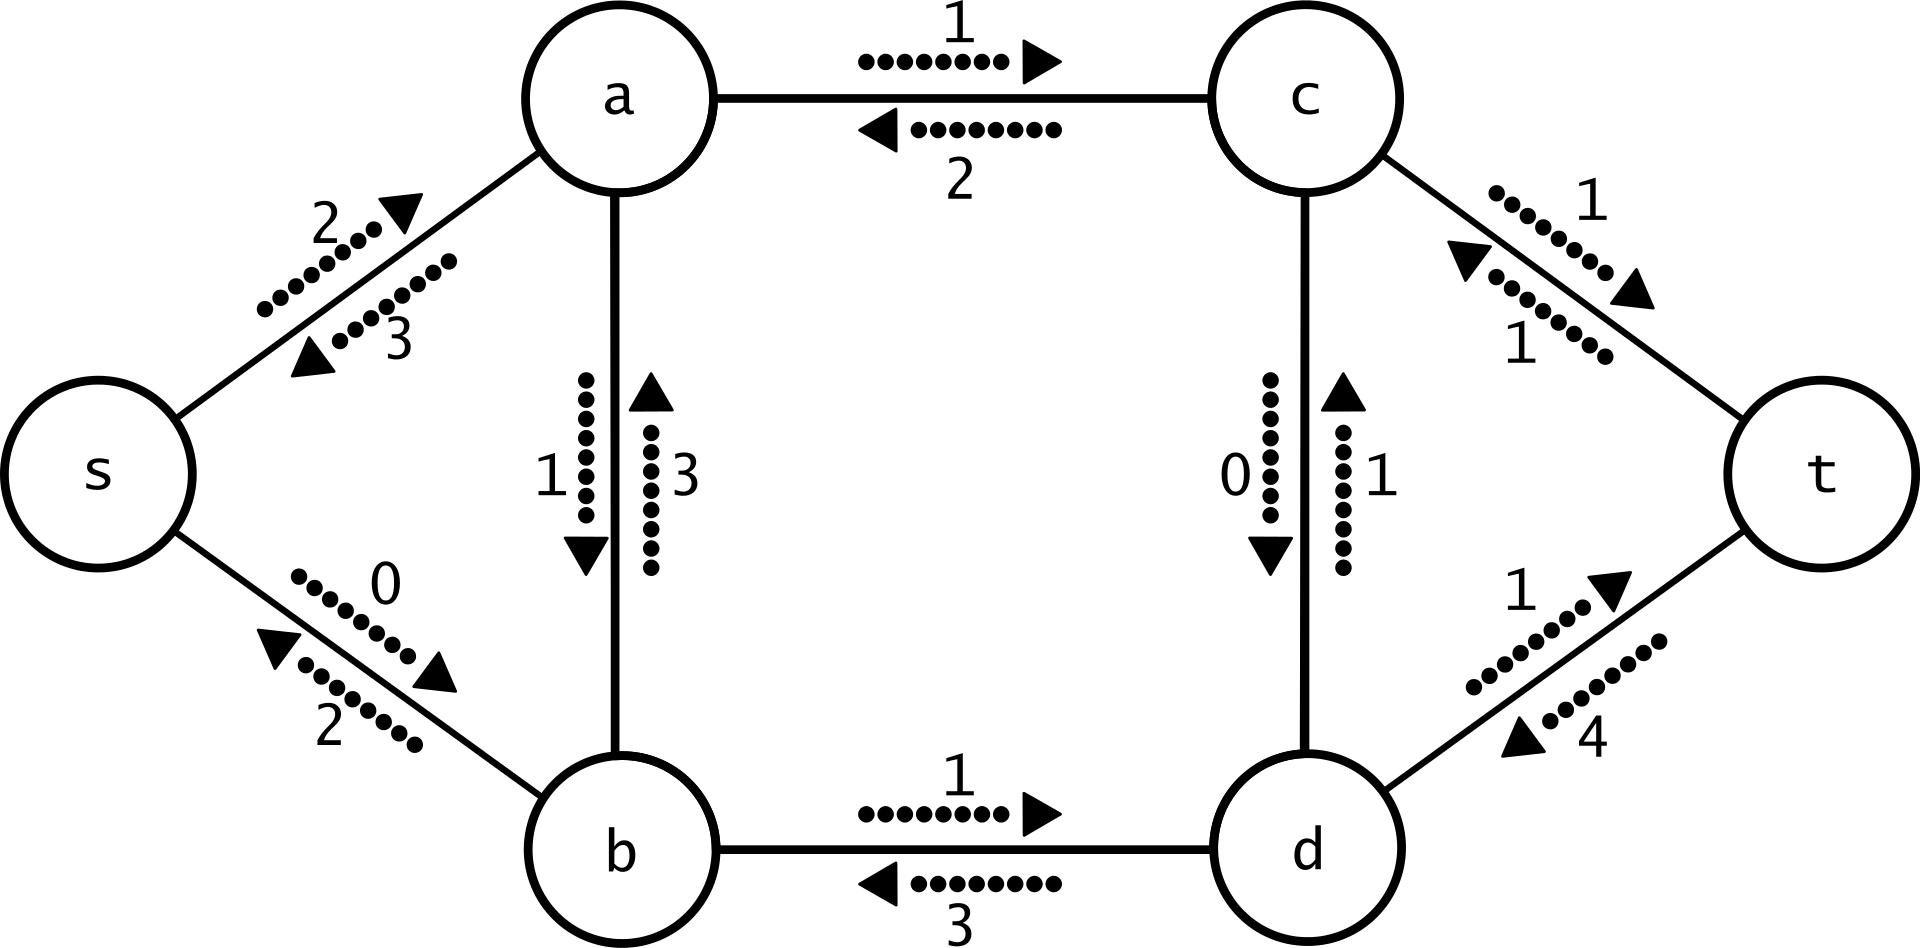
\includegraphics[scale=.06]{residual.png}
\end{center}

\subsubsection*{Max Flow Min Cut Theorem}
The size of the maximum flow in a network equals the capacity of the smallest (s,t)-cut, where and (s,t)-cut partitions the vertices into two disjoint groups L and R such that s (start) is in L and t (goal) is in R.

\subsubsection*{Bipartite Matching}
Explained by Example: list of boys, list of girls, if boy likes girl, a direct edge exists from boy to girl. Is there a perfect matching?
Create source node $s$ and sink node $t$, $s$ has outgoing edges to all the boys, and $t$ has incoming edges from all the girls. Give every edge a capacity of one (obviously). A flow exists if there is a flow into $t$ with size equal to number of couples. 

%%%%%%%%%%%%%%%%%%%%%%%%%

\section*{Computational Complexity}
We use Computational Complexity to determine classifications for our algorithms to know if they are feasible. 

\subsection*{Decision vs. Search Problems}
\textbf{Decision Problem: }Computational problem that answers ``Yes'' or ``No''. Our input can be any possible string (binary, ASCII), and it will answer either 0 or 1 depending upon weather the solution is correct or not. This type of problem determines our classes.\\
\textbf{Search Problem: }Computational problem tasked with not if a solution exists, but what one is. Decision problems can be derived from Search problems which are generally always more difficult. 

\subsection*{Classifications}
\begin{itemize}
\item \textbf{P}: The set of all search problems that are solvable in a reasonable amount of time (Polynomial time).
\item \textbf{NP (Nondeterministic Polynomial)}: The set of all search problems whose solution can be checked in Polynomial time (includes P) - there might exist search problems whose solutions can not be checked in Polynomial time. A solution may not necessary be found in a reasonable amount of time ($2^n$ and $n!$ algorithms can be in NP). Called NP because if you had the power to guess correct every time it would work in Polynomial time, making it non-deterministic. Should be called ``Guessing in P''.
\item \textbf{NP-Hard:} Any problem in NP can be reduced to this problem in Polynomial time, so it is at least as difficult or ``hard'' as any NP problem. The Halting Problem is NP hard and also impossible to solve in a finite amount of time, so this idea is not always practically useful for reductions. Most NP-Hard problem are NOT in NP, but those that are, are NP-Complete.
\item \textbf{NP-Complete: }Problem that is not only as hard as every problem in NP, but is also in NP. (NP-Hard and in NP). Any NP problem can be reduced to one of these in Polynomial time. It is often useful to prove the difficulty of problems. These are the hardest problems in NP and the reason why P = NP can revolutionize things. 
\end{itemize}
\begin{center}
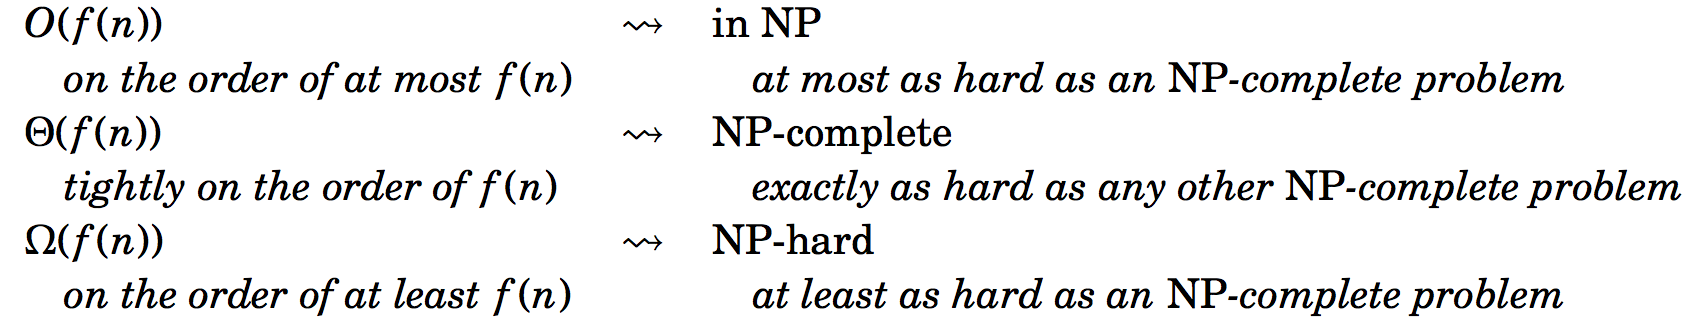
\includegraphics[scale=.25]{analogy.png}
\end{center}

\subsection*{Common NP-Complete Problems}
\begin{center}
\begin{tabular}{|c|c|}
    \hline
    Hard problems(NP-complete) & Easy problems (in P)\\
    \hline
    \hline
    3SAT & 2SAT, HORN SAT\\
    Traveling Salesman Problem & Minimum Spanning Tree\\
    Longest Path & Shortest Path\\
    3D Matching & Bipartite Matching\\
    Knapsack & Unary Knapsack\\
    Independent Set & Independent Set on trees\\
    Integer Linear Programming & Linear Programming\\
    Rudrata Path & Euler Path\\
    Balanced Cut & Minimum Cut\\
    \hline
\end{tabular}
\end{center}

\subsubsection*{Satisfiability (SAT)}
This is the prototypical NP-Complete problem that everything started from.
Say you have some Boolean expressions written using only AND, OR, NOT, variables, and parentheses (Example: $x_1 \land x_2 \lor x_3$). The SAT problem is given any one of these expressions, is there some assignment of TRUE and FALSE values to the variables that will make the entire expression TRUE? 
\subsubsection*{3SAT}
This is a stricter version of the SAT problem in which the statement is divided into clauses where each clause can have exactly 3 literals. (Example: $(x_1 \lor x_2 \lor x_3)\land(x_4 \lor x_5 \lor x_6)$). For these you want to find whether there exists values for $x_1 ... x_6$such that the boolean evaluates to TRUE.
\subsubsection*{CircuitSAT}
Given a circuit of logic gates with a single output and no loops find there a setting of the inputs that causes the circuit to output 1.
\subsubsection*{Integer Linear Programming} 
Solve a problem using linear objective function and linear inequalities, WHILE constraining the values of the variables to integers. 
\subsubsection*{Traveling Salesman Problem (TSP)}
Find the \textit{shortest path} in a graph that visits all the vertices exactly once before returning home. This comes from the idea of a traveling salesman wanting to efficiently visit all the cities to sell his wares. 
\subsubsection*{Rudrata/Hamiltonian Cycle}
Given a graph find if there a cycle that passes through each vertex exactly once, or report one doesn't exist. 
\subsubsection*{Rudrata/Hamiltonian Path}
Given a path starting at $s$ and ending at $t$ that goes through each vertex exactly once.
\subsubsection*{Independent Set}
Given a graph and a number $g$, the aim is to find $g$ vertices that are independent meaning that no two of which have share an edge. 
\subsubsection*{Graph 3-Coloring}
Given an undirected graph G = (V,E) find a valid 3-coloring C such that no two vertices sharing the same edge have the same color, or report that such an ordering doesn't exist. 


%%%%%%%%%%%%%%%%%%%%%%%%%

\section*{Reductions}
Reductions are an incredible useful tool for either turning a search problem we don't know how to solve into one we do, or proving that a search problem can not be solved or is hard to solve by reducing it to problem that is one of those two things.\\
- We know how to solve $B$ in a reasonable amount of time and we want to use this knowledge to solve $A$.\\
- We denote a reduction from $A$ to $B$ as $A \to B$. Difficultly flows in the direction of the arrow.\\
- If we can reduce our unknown problem $A$ into a known problem $B$ then $B$ must be as hard if not even harder to solve than $A$. A way to mathematically write this is $A \le_{p} B$. $A$ thereby provides a lower bound of hardness for $B$.\\ 
- Reduction can be composed as well: if you can reduce $A \to B$ and $B \to C$ then $A \to C$.\\
- Any search problem in NP can be reduced to an NP-Hard Problem in Polynomial Time but this is not always useful (like Halting Problem) \\
- Any search problem in NP can also be reduced to an NP-Complete Problem in Polynomial Time.\\
- Any problem that is NP-Complete is reducible to any other problem that is also NP-Complete which is very useful.
\subsubsection*{Reduction Tree}
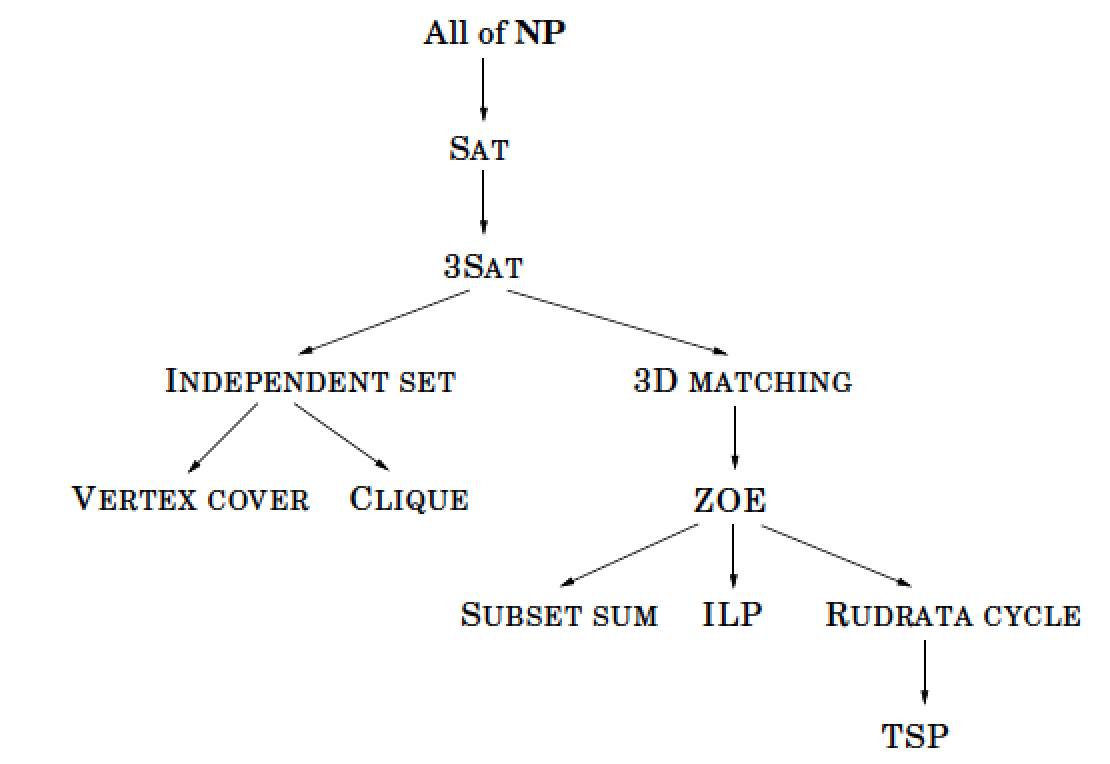
\includegraphics[scale=.4]{reductions.png}



%\rule{0.3\linewidth}{0.1pt}
\scriptsize

\end{multicols}
\end{document}